%% LaTeX2e class for student theses
%% thesis.tex
%% 
%% Karlsruhe Institute of Technology
%% Institute for Program Structures and Data Organization
%% Chair for Software Design and Quality (SDQ)
%%
%% Dr.-Ing. Erik Burger
%% burger@kit.edu
%%
%% See https://sdq.kastel.kit.edu/wiki/Dokumentvorlagen
%%
%% Version 1.4, 2023-06-19

%% Available page modes: oneside, twoside
%% Available languages: english, ngerman
%% Available modes: draft, final (see README)
\documentclass[twoside, english, draft]{sdqthesis}

\usepackage[nocn]{ffcode}
\usepackage{csquotes}
\usepackage{float}

\ifdraft{
\usepackage{draftwatermark}
\SetWatermarkAngle{50}
\SetWatermarkLightness{0.9}
\SetWatermarkScale{1}
\usepackage{todonotes}
}{}


%% ---------------------------------
%% | Information about the thesis  |
%% ---------------------------------

%% Name of the author
\author{Lars Weber}

%% Title (and possibly subtitle) of the thesis
\title{Generation of Checkpoints for Hardware Architecture Simulators}

%% Type of the thesis 
\thesistype{Bachelor's Thesis}

%% Change the institute here, ``KASTEL'' is default
% \myinstitute{Institute for \dots}

%% You can put a logo in the ``logos'' directory and include it here
%% instead of the SDQ logo
% \grouplogo{myfile}
%% Alternatively, you can disable the group logo
% \nogrouplogo

%% The reviewers are the professors that grade your thesis
\reviewerone{PD. Dr. Robert Heinrich}
\reviewertwo{Prof. Dr. Ralf H. Reussner}

%% The advisors are PhDs or Postdocs
\advisorone{M. Sc. Sebastian Weber}
%% The second advisor can be omitted
\advisortwo{PD. Dr. Robert Heinrich}

%% Please enter the start end end time of your thesis
\editingtime{13. Mai 2024}{13. September 2024}

\settitle

%% --------------------------------
%% | Bibliography                 |
%% --------------------------------

%% Use biber instead of BibTeX, see README
\usepackage[citestyle=numeric,style=numeric,backend=biber]{biblatex}
\addbibresource{thesis.bib}

%% For example texts -- please remove in the final version
\usepackage{blindtext}

%% ====================================
%% ====================================
%% ||                                ||
%% || Beginning of the main document ||
%% ||                                ||
%% ====================================
%% ====================================
\begin{document}

\newcommand{\todonote}[1]{\ifdraft{
\todo{#1}
}{}}

%% Set PDF metadata
\setpdf

%% Set the title
\maketitle

%% The Preamble begins here
\frontmatter

%% LaTeX2e class for student theses: Declaration of independent work
%% sections/declaration.tex
%% 
%% Karlsruhe Institute of Technology
%% Institute for Program Structures and Data Organization
%% Chair for Software Design and Quality (SDQ)
%%
%% Dr.-Ing. Erik Burger
%% burger@kit.edu
%%
%% Version 1.3.3, 2018-04-17

\thispagestyle{empty}
\null\vfill
\noindent\hbox to \textwidth{\hrulefill} 
\iflanguage{english}{I declare that I have developed and written the enclosed
thesis completely by myself, and have not used sources or means without
declaration in the text.}%
{Ich versichere wahrheitsgemäß, die Arbeit
selbstständig angefertigt, alle benutzten Hilfsmittel vollständig und genau
angegeben und alles kenntlich gemacht zu haben, was aus Arbeiten anderer
unverändert oder mit Änderungen entnommen wurde.}
 
 
%% ---------------------------------------------
%% | Replace PLACE and DATE with actual values |
%% ---------------------------------------------
\textbf{PLACE, DATE}
\vspace{1.5cm}
 
\dotfill\hspace*{8.0cm}\\
\hspace*{2cm}(\theauthor) 
\cleardoublepage

\setcounter{page}{1}
\pagenumbering{roman}

%% ----------------
%% |   Abstract   |
%% ----------------
 
%% For theses written in English, an abstract both in English
%% and German is mandatory.
%%
%% For theses written in German, a German abstract is sufficient.
%%
%% The text is included from the following files:
%% - sections/abstract

\includeabstract

%% ------------------------
%% |   Table of Contents  |
%% ------------------------
\tableofcontents

\listoffigures
\listoftables

%% -----------------
%% |   Main part   |
%% -----------------

\mainmatter

%% LaTeX2e class for student theses
%% sections/content.tex
%% 
%% Karlsruhe Institute of Technology
%% Institute for Program Structures and Data Organization
%% Chair for Software Design and Quality (SDQ)
%%
%% Dr.-Ing. Erik Burger
%% burger@kit.edu
%%
%% Version 1.5, 2024-02-12

\chapter{Introduction}\label{chap:introduction}
The planning and development of large-scale software infrastructures often encompasses software distributed over many different devices,
which may feature vastly different environments for the code running on them.
Especially devices "out in the field" regularly feature architectures very different from the specifications of x86 or ARM,
which makes them very difficult to predict in system simulations or generally in the early planning stages.
Especially when planning real-time systems,
it is very important to plan the communication between IoT devices and the servers running in the backend.
In these scenarios, the backend often runs on x86, or in more recently implemented systems ARM,
while the external devices feature all kinds of different architectures,
that are usually specialized to the task at hand.
Even many IoT devices running ARM cores can often not easily be compared to smartphone- or server-grade ARM.
In addition, when modifying such systems, for example when upgrading hardware,
many of these specialized architectures feature certain behaviors that may be unexpected or not well documented,
which must be addressed when swapping out these physical parts.

In the actual development phase, this issue is already getting solved using emulation.
In the planning phase, especially during design space exploration, where small experiments are already being run,
certain external software is already available, or if the project is a switch of architectures,
like from x86 to ARM in the server world,
emulation could also be used to offer more detailed planning
like for performance criteria.
When a server in a data center is supposed to communicate with an external part that uses pre-developed software,
such an emulation can now be used to produce a good estimate of how performant the server needs to be and how long it should expect to wait for replies.
However, there are issues with emulation, which hinder the use of it in these stages.
The biggest of which is speed, as emulation may result in a slowdown of the factor 1000-10000\cite{slowdown}.
Especially during the exploration of the design space, where only the outline of the project needs to be put down,
such a slowdown is unacceptable, considering the results of the simulation don't need to be exact.

As there are many different emulation environments available,
this thesis chose QEMU, as it is open source and has the most resources available to work with.
The details of the process which led to the selection of QEMU are detailed in \autoref{sec:emulators}.
This thesis tries to generalize findings that may be transferred to other environments,
however as all of these are heavily specialized tools,
the amount of transferrable findings is very limited.

This thesis now introduces the idea of checkpoints to solve this issue of speed and associated resource costs.
The idea is to extract all relevant data from a running emulation
and store it in a generalized way which allows for reusal of the saved state of the system in a different context.
The goal here is to provide a solution with as much flexibility as possible,
meaning a tool which does not require manual tweaking depending on the targeted system.
This especially involves a version-independence in regards to the emulator used.
QEMU has featured the QEMU Human Monitor (QHM) for a long time,
it is however explicitly not meant for processing by other software.
To allow interaction with other software, the QEMU Machine Protocol (QMP) was developed, and the goal is to use this protocol instead,
as the QEMU team tries to keep it somewhat standardized,
while they explicitly write QHM is not stable and there is no guarantee its used formats will be kept consistent,
especially for usages that are not typical for the normal user.
The differences and limitations of both protocols are discussed in detail in \autoref{chap:QEMU_API}.

Initially, this research also aimed to make the development of embedded software easier by using emulation checkpoints to speed up development.
As mentioned before, emulation is very slow.
This of course still applies during development, especially when there is not yet a physical prototype of the developed system available.
To achieve a speedup here, the idea was to make the checkpoints reusable
and create the ability to inject already existing checkpoints back into a running emulation.
This would have even given the option to calculate checkpoints centrally and distribute them,
to save on time and especially resources.
This behavior could not be implemented because of the  limitations of QEMU,
more details on this can be read in \autoref{sec:injection}.
In case someone intends to build up on this and implement the re-injection,
they will find all information regarding such functionality found during this research there.

The theoretical outlines of this thesis including definitions used as well as other works in this field are included in \autoref{chap:Foundations}.
\autoref{chap:QEMU_API} contains both a description of the QEMU APIs according to their official documentation,
however also findings by myself as the official documentation is quite lacking in certain parts, especially the documentation about QHM.
For this reason, it was also decided to make it into its own chapter.
The implementation itself as well as challenges faced during it are mentioned in \autoref{chap:implementation},
and the results of this implementation are discussed and evaluated in \autoref{chap:Evaluation}.
Finally, the works and results of this thesis are concluded in \autoref{chap:Conclusion}.
%% LaTeX2e class for student theses
%% sections/content.tex
%% 
%% Karlsruhe Institute of Technology
%% Institute of Information Security and Dependability
%% Software Design and Quality (SDQ)
%%
%% Dr.-Ing. Erik Burger
%% burger@kit.edu
%%
%% Version 1.5, 2024-02-12

\chapter{The QEMU API} \label{chap:QEMU_API}
As the goal of this thesis is to extract data without having to change the code of QEMU,
it is necessary to take a look at the data QEMU offers by itself.
QEMU offers 3 kinds of semi-external APIs: The QEMU Human Monitor (QHM)\cite{qhm-documentation},
the QEMU Machine Protocol (QMP)\cite{qmp-description} and so-called "Internal QEMU APIs"\cite{internal}.

As the name suggests, the internal QEMU APIs are not useful for external use by themselves.
Instead, they can be used when modifying QEMU code and then extracting data by employing GDB or directly by the QEMU process.
As the goal is to use any standard QEMU implementation, these internal APIs will not be regarded further in this thesis.

In the two following sections, both QMP and QHM are further explored. Both the basic functionality,
as well as the commands used for this thesis are explained in detail.
Also, the differences between both protocols, especially regarding their capabilities,
are discussed.

\section{QEMU Machine Protocol (QMP)} \label{sec:QMP}
\enquote{The QEMU Machine Protocol (QMP) is a JSON-based protocol which allows applications to control a QEMU instance}\cite{qmp-description}, as described in the QEMU Wiki.
The protocol was merged into the main branch of QEMU in version 0.13 in 2010, however to this day its status remains as "experimental"\cite{qmp-merge}.
The goal was, and still is, to provide the same data QHM provides, but in a format more accessible for machines.

However, this process is far from complete. To give an example, the patch to add the ability to read register contents was only introduced in 2021,
but to this day it hasn't been merged into the mainline branch.
In addition, this patch doesn't actually provide a valid JSON object, but just passes the return of the QHM-command "info registers" into the "result"-string\cite{qmp-registers-patch},
which is also the reason why it was not merged, as it would have been in conflict with the goal of making QMP both machine-readable and externally consistent.

This effectively means QMP is the preferred protocol for performing any given task,
since its outputs are easily parseable and the QEMU team tries to keep them consistent.
However, there are many tasks QMP cannot (yet) perform,
so certain tasks require the usage of QHM for lack of QMP support.
This directly leads to the most important command\cite{qmp-commands}:

\paragraph{human-monitor-command}
This command is rather special, as it doesn't provide any information by itself,
but instead allows for usage of the legacy QHM inside of QMP,
which gives access to a lot more data not yet accessible directly in QMP.
The QEMU reference explicitly marks this command as a \enquote{stop-gap} until all QHM-commands have their counterpart in QMP,
but, as mentioned before, that is not a priority at the moment.
Still, it's currently the only way to access certain data like register contents, even if the results require extensive and complicated parsing.
Further details on how this command is used and what its capabilities are are described later on in \autoref{sec:QHM}.

\paragraph{qmp\_capabilities}
This command must be sent at the beginning of any QMP session to activate the session.
On an unmodified QEMU instance, it returns an empty JSON object.
The command is intended to show the client additional features of a modified QEMU-instance,
however in this thesis this command serves no purpose except unlocking QMP.

\paragraph{query-cpus-fast}
Gives information about all available CPUs, namely their architecture,
their count, and the ID of the host thread simulating the CPU.
The command is a replacement for \emph{query-cpus}, which was removed and returned slightly different data.
The main purpose this command serves for this thesis is to get the CPU count,
as registers need to be queried individually for each CPU.

\paragraph{query-block}
Queries for all kinds of drives. Gives information about attached storage mediums and where their content is stored.
This gets used to back up the necessary files later on.
Also shows empty devices like optical drives which currently don't contain any media.

\paragraph{dump-guest-memory}\label{dump_memory}
This command dumps the contents of the guest's memory to disk.
The command itself offers many options, however most of these don't work.
In the used implementation, the only output format working is ELF, and paging is only possible on x86 guests.
Still, it's the only option in QMP that offers access to the guest's memory.

\paragraph{stop}
Suspends the emulation of the current system. It is necessary to keep the data extracted consistent.

\paragraph{cont}
Continues the execution of a previously paused system.

\section{QEMU Human Monitor (QHM)} \label{sec:QHM}
The QEMU Human Monitor, sometimes referred to as only the QEMU Monitor,
is an interface to send commands to and query data from a running QEMU instance in a human-readable form.
This however often leads to inconsistent representation, as there is no clear standard on how to represent data.
Even within single commands, the format may vary wildly across different architectures or even within the same architecture.
At the same time, documentation of commands is very lacking, sometimes consisting of only a single sentence.
This makes a detailed exploration into their workings necessary, and the results of this research are presented in the following\cite{qhm-documentation}:

\subsection{info tlb}
"info tlb" is described as "Show virtual to physical memory mappings"\cite{qhm-documentation}.
There seems to be no further documentation as to what this command does or the format of the output.
Finding more information about the supposed TLB is also rather difficult.
Most information is therefore derived from the \citetitle{intel-manual},
which therefore only applies to x86 and makes the portability of any information rather questionable.

An example of the output is provided in \autoref{fig:tlb_x86}:

\begin{figure}[H]
\begin{ffcode}
    0000000000010000: 00000000001a0000 ---DA---W
    0000000000011000: 0000000000181000 ---DA---W
    0000000000012000: 0000000000182000 ---DA---W
    0000000000013000: 0000000000183000 ---DA---W
    0000000000014000: 0000000000184000 ---DA---W
    0000000000015000: 0000000000185000 ----A---W
    0000000000016000: 0000000000186000 ---DA----
    0000000000017000: 0000000000187000 ----A---W
    0000000000018000: 0000000000188000 ----A----
    0000000000019000: 0000000000189000 ----A----
    000000000001a000: 000000000016a000 ----A----
\end{ffcode}
\caption{Output of \emph{info tlb}.}
\label{fig:tlb_x86}
\end{figure}

These are the first eleven lines this command outputs when queried against the XBox emulator "xemu"\cite{xemu}.
The output consists of the linear address shown to the guest OS, the "physical" address, which represents the offset in QEMU's emulated memory region,
and the flags associated with each segment.
As the flags are x86-specific, they are currently not of further interest and just get stored without further processing.

It is important to note the physical address is not the actual address in the QEMU process, but the offset from the base address of said memory region.
To correctly extract the guest RAM, one would now need to find the base address of the memory region the QEMU-process uses to emulate RAM,
and then combine it with the virtual address translation to store memory in the format the guest OS sees it.
This throws up the question of which format the RAM should be stored. In the order it is actually on the hardware, meaning the physical addresses,
or in the order the guest OS sees it, meaning the virtual addresses.

\subsection{info mtree}\label{sec:API_mtree}
This command shows all memory regions which are currently allocated for the guest.
This includes main memory, as well as memory for emulated devices like graphic cards.
These regions are given individual names and are separated by blank lines.
\autoref{fig:mem_ARM} gives an excerpt of an ARM64 guest running on x86,
the full output is shown in \autoref{fig:mem_ARM_full}.

\begin{figure}[H]
\begin{ffcode}
    address-space: I/O
    0000000000000000-000000000000ffff (prio 0, i/o): io

  address-space: gpex-root
    0000000000000000-ffffffffffffffff (prio 0, i/o): bus master container

  address-space: virtio-gpu-pci
    0000000000000000-ffffffffffffffff (prio 0, i/o): bus master container

  address-space: cpu-memory-0
  address-space: memory
    0000000000000000-ffffffffffffffff (prio 0, i/o): system
      0000000000000000-0000000003ffffff (prio 0, romd): virt.flash0
      0000000004000000-0000000007ffffff (prio 0, romd): virt.flash1
      0000000008000000-0000000008000fff (prio 0, i/o): gic_dist
      0000000008010000-0000000008011fff (prio 0, i/o): gic_cpu
      0000000008020000-0000000008020fff (prio 0, i/o): gicv2m
      0000000009000000-0000000009000fff (prio 0, i/o): pl011
      0000000009010000-0000000009010fff (prio 0, i/o): pl031
      0000000009020000-0000000009020007 (prio 0, i/o): fwcfg.data
      0000000009020008-0000000009020009 (prio 0, i/o): fwcfg.ctl
      0000000009020010-0000000009020017 (prio 0, i/o): fwcfg.dma
      0000000009070000-0000000009070017 (prio 0, i/o): memhp container
      0000000009080000-0000000009080003 (prio 0, i/o): acpi-ged
      000000000a000000-000000000a0001ff (prio 0, i/o): virtio-mmio
      000000000a000200-000000000a0003ff (prio 0, i/o): virtio-mmio
      000000000a000400-000000000a0005ff (prio 0, i/o): virtio-mmio
      ...
\end{ffcode}
\caption{Output of \emph{info mtree} for an ARM guest.}
\label{fig:mem_ARM}
\end{figure}

In this example, we see memory for basic I/O functionality, the GPEX-host bridge, the emulated GPU, and "cpu-memory-0".
cpu-memory-0 is special, as the name suggests this may be memory used to emulate the CPU. That however is not the case.
Not only is it much larger than the registers of a single-core CPU could be, but also it's a duplicate.
Further down the output is the following data:

\begin{figure}[H]
\begin{ffcode}
    memory-region: system
    0000000000000000-ffffffffffffffff (prio 0, i/o): system
      0000000000000000-0000000003ffffff (prio 0, romd): virt.flash0
      0000000004000000-0000000007ffffff (prio 0, romd): virt.flash1
      0000000008000000-0000000008000fff (prio 0, i/o): gic_dist
      0000000008010000-0000000008011fff (prio 0, i/o): gic_cpu
      0000000008020000-0000000008020fff (prio 0, i/o): gicv2m
      0000000009000000-0000000009000fff (prio 0, i/o): pl011
      0000000009010000-0000000009010fff (prio 0, i/o): pl031
      0000000009020000-0000000009020007 (prio 0, i/o): fwcfg.data
      0000000009020008-0000000009020009 (prio 0, i/o): fwcfg.ctl
      0000000009020010-0000000009020017 (prio 0, i/o): fwcfg.dma
      0000000009070000-0000000009070017 (prio 0, i/o): memhp container
      0000000009080000-0000000009080003 (prio 0, i/o): acpi-ged
      000000000a000000-000000000a0001ff (prio 0, i/o): virtio-mmio
      000000000a000200-000000000a0003ff (prio 0, i/o): virtio-mmio
      000000000a000400-000000000a0005ff (prio 0, i/o): virtio-mmio
      ...
\end{ffcode}
\caption{Duplicate data for \emph{info mtree} on an ARM guest.}
\label{fig:mem-duplicate}
\end{figure}

This shows that the output above is actually normal system memory accessible to the emulated CPU.
Hence the name "cpu-memory-0", as on multi-socket-systems sometimes not all memory is available to all CPUs.

The size of each memory region is shown by the minimum and maximum address of each region.
As this is a 64bit guest, ffffffffffffffff represents 64bits, which results in a memory size of $2^{64}$Bytes.

Most regions are specialized and the name of the region gives an indication of where to look,
but it isn't actually relevant in most cases.
Because of this, only one special region will be explained:

\paragraph{virt.flash}
There are 2 regions with this name. \emph{virt.flash0} is the basic EFI, which under aarch64 is not included by default.
\emph{virt.flash1} stores EFI variables like the boot order.
The reason these regions are split is \emph{virt.flash1} is writeable, while \emph{virt.flash0} isn't.
The main reason these are interesting is them being backed by files on disk.
This means any changes made to these regions by the guest can be easily read externally by opening those files.
Of course that comes with a massive performance penalty if many accesses to such regions are made.

Additionally, since x86 is often more detailed than other architectures,
the full output of \emph{info mtree} is also shown in \autoref{fig:xemu_full}.

\subsection{info registers}\label{sec:info_registers}
This command returns the contents of all the registers for a given CPU.
It gives a detailed overview of the data, however the level of detail on x86 is much higher than it is for other architectures.
To further illustrate this, in \autoref{fig:registers_x86} and \autoref{fig:registers_ARM} example outputs for this command are provided.

\begin{figure}[H]
  \begin{ffcode}
    CPU#0
    EAX=fd000140 EBX=80035bdc ECX=fd601300 EDX=00000000
    ESI=80035a90 EDI=d0008bf8 EBP=80035c2c ESP=800395f0
    EIP=8001b030 EFL=00000246 [---Z-P-] CPL=0 II=0 A20=1 SMM=0 HLT=0
    ES =0010 00000000 ffffffff 00cf9300 DPL=0 DS   [-WA]
    CS =0008 00000000 bfffffff 00cb9b00 DPL=0 CS32 [-RA]
    SS =0010 00000000 ffffffff 00cf9300 DPL=0 DS   [-WA]
    DS =0010 00000000 ffffffff 00cf9300 DPL=0 DS   [-WA]
    FS =0020 80035bdc 0027cfff 00c09300 DPL=0 DS   [-WA]
    GS =0000 00000000 00000000 00000000
    LDT=0000 00000000 0000ffff 00008200 DPL=0 LDT
    TR =0018 8003b160 00000068 00008900 DPL=0 TSS32-avl
    GDT=     8003b298 00000038
    IDT=     80035e60 00000200
    CR0=8001003b CR2=00000000 CR3=0000f000 CR4=00000610
    DR0=00000000 DR1=00000000 DR2=00000000 DR3=00000000
    DR6=ffff0ff0 DR7=00000400
    EFER=0000000000000000
    FCW=027f FSW=0000 [ST=0] FTW=00 MXCSR=00001fa0
    FPR0=0000000000000000 0000 FPR1=0000000000000000 0000
    FPR2=0000000000000000 0000 FPR3=0000000000000000 0000
    FPR4=0000000000000000 0000 FPR5=0000000000000000 0000
    FPR6=0000000000000000 0000 FPR7=0000000000000000 0000
    XMM00=0000000000000000 0000000041080000 XMM01=0000000000000000 000000004f000000
    XMM02=0000000000000000 00000000cf000000 XMM03=0000000000000000 0000000043a00000
    XMM04=0000000000000000 0000000000000000 XMM05=0000000000000000 0000000000000000
    XMM06=0000000000000000 0000000000000000 XMM07=0000000000000000 0000000000000000
  \end{ffcode}
  \caption{Example Output of \emph{info registers} on an x86 guest.}
  \label{fig:registers_x86}
\end{figure}

\begin{figure}[H]
  \begin{ffcode}
    CPU#0
    PC=0000000000000200 X00=0000000000000000 X01=0000000000000000
    X02=0000000000000000 X03=0000000000000000 X04=0000000000000000
    X05=0000000000000000 X06=0000000000000000 X07=0000000000000000
    X08=0000000000000000 X09=0000000000000000 X10=0000000000000000
    X11=0000000000000000 X12=0000000000000000 X13=0000000000000000
    X14=0000000000000000 X15=0000000000000000 X16=0000000000000000
    X17=0000000000000000 X18=0000000000000000 X19=0000000000000000
    X20=0000000000000000 X21=0000000000000000 X22=0000000000000000
    X23=0000000000000000 X24=0000000000000000 X25=0000000000000000
    X26=0000000000000000 X27=0000000000000000 X28=0000000000000000
    X29=0000000000000000 X30=0000000000000000  SP=0000000000000000
    PSTATE=000003c5 ---- EL1h  SVCR=00000000 --  BTYPE=0    FPU disabled
  \end{ffcode}
  \caption{Example output of \emph{info registers} on an ARM guest.}
  \label{fig:registers_ARM}
\end{figure}

It is immediately apparent this output is not intended for further usage by computers,
but instead used by humans debugging QEMU and does not follow any specified format.
This of course is also stated by the QEMU team\cite{qhm-documentation}.
However, because this is the only way to access registers through an external interface,
this output needs to be made parseable by a computer, and for this,
the following rules are presumed from ARM and x86 in the hope they are valid for the majority of architectures:

\begin{itemize}
  \item The CPU number is specified in the first line, even though the command only returns a single CPU which must be specified beforehand.
  \item Registers are formatted in the scheme \$name=\$content.
  \begin{itemize}
    \item On x86, if the name of the register is shorter than 3 letters, the name gets padded with spaces between it and the equals sign.
    \item Longer names are allowed, however as the names of most standard registers are only 3 letters long, this only applies to more specialized registers.
    \item The content is specified in hexadecimal.
  \end{itemize}
  \item The length of the content gets padded with zeroes at the beginning to indicate the length of the register.
  Since this is in hex, each digit represents 4 bits of register length.
  \begin{itemize}
    \item This assumes all registers are of a length divisible by four.
    However, there are registers where this is not the case, for example $HLT$ or $A20$.
  \end{itemize}
  \item QEMU formats the contents into groups of \emph{some} multiple of 32 bits.
  \begin{itemize}
    \item When the amount of bits in a register is not a multiple of \emph{some} multiple of 32,
    there is no standard whether the remaining bits get put at the back or the front.
    See the floating-point and stack-pointer registers.
  \end{itemize}
  \item 3 different ways to represent flags were encountered:
  \begin{enumerate}
    \item Some flags get put in []-brackets, wherein their letter is written if they're set, otherwise a hyphen is shown.
    \item Other flags, especially multibit flags, get represented like their own register.
    \begin{itemize}
      \item In this case, the amount of digits does not indicate the length of the register and therefore its possible values.
      For example, the $A20$-register is only a single bit, while $CPL$ is 2 bits.
    \end{itemize}
    \item If there is not a dedicated register in the specification,
    but it's up to the implementation to decide,
    for example the FPU on ARM,
    there is no standard in how this is treated.
    \begin{itemize}
      \item For the ARM-FPU, \enquote{FPU disabled} gets explicitly written out,
      while on x86 such information is stored in the specified registers and represented using a 0 or a 1.
      \item There was no attempt to explicitly search for occurrences of this case,
      as the implementation of these cases is specific to the architecture in question
      and there exists no documentation of such cases.
    \end{itemize}
  \end{enumerate}
  \item The targeted line length seems to be 50 around symbols.
  \item Inside a group of registers with the same or similar purpose, the formatting seems to be somewhat consistent.
  \begin{itemize}
    \item The general purpose and the control registers feature 4 registers per line,
    the pointer registers one register per line, the floating point and SIMD registers show 2 registers per line.
    \item The pointer registers apparently aim to keep full blocks of 32 bits aligned,
    meaning the $GDT$ and $IDT$ registers have their content shifted to the right by 5 places so they align with the first full 32 bit of the other registers.
    \item The flags associated with the general purpose registers are simply appended to the registers.
    Instead, the registers for special CPU features like $EFER$ are written in their own respective lines.
    The flags for pointer registers get written in the same line as the respective register,
    which is also the only way of finding out which flag is associated with which register.
  \end{itemize}
\end{itemize}

\subsection{memsave \& pmemsave}\label{sec:memsave}
These commands are the ancestors to \emph{dump-guest-memory} in \autoref{dump_memory}.
They are far less sophisticated than their QMP successor,
which means they should not be used anymore.
However, they do allow for quick and easy testing,
as they simply create a raw memory dump without any additional metadata.
When actually extracting data from QEMU, such metadata is of course very helpful,
but during debugging these 2 commands are a lot easier to use.
Also, because of this simplicity, there is no special behavior in need of mentioning.

They also allow for the direct separation of physical and virtual memory,
which requires explicit parsing for \emph{dump-guest-memory}.
This also means that \emph{memsave} is only available on guests which allow for paging on \emph{dump-guest-memory},
meaning currently only x86 is supported.
\emph{pmemsave} is available on all platforms, however as it's physical memory,
it is a bit harder to make sense of the data.
%% LaTeX2e class for student theses
%% sections/evaluation.tex
%% 
%% Karlsruhe Institute of Technology
%% Institute for Program Structures and Data Organization
%% Chair for Software Design and Quality (SDQ)
%%
%% Dr.-Ing. Erik Burger
%% burger@kit.edu
%%
%% Version 1.3.3, 2018-04-17

\chapter{Evaluation}
\label{ch:Evaluation}

%% -------------------
%% | Example content |
%% -------------------
\dots

\section{First Section}
\label{sec:Evaluation:FirstSection}

\dots

\section{Second Section}
\label{sec:Evaluation:SecondSection}

\dots

\section{Third Section}
\label{sec:Evaluation:ThirdSection}

\dots
%% ---------------------
%% | / Example content |
%% ---------------------
%% LaTeX2e class for student theses
%% sections/conclusion.tex
%% 
%% Karlsruhe Institute of Technology
%% Institute for Program Structures and Data Organization
%% Chair for Software Design and Quality (SDQ)
%%
%% Dr.-Ing. Erik Burger
%% burger@kit.edu
%%
%% Version 1.3.5, 2020-06-26

\chapter{Conclusion}
\label{ch:Conclusion}

\dots

%% --------------------
%% |   Bibliography   |
%% --------------------

%% Add entry to the table of contents for the bibliography
\printbibliography[heading=bibintoc]

%% ----------------
%% |   Appendix   |
%% ----------------
\appendix
%% LaTeX2e class for student theses
%% sections/apendix.tex
%% 
%% Karlsruhe Institute of Technology
%% Institute of Information Security and Dependability
%% Software Design and Quality (SDQ)
%%
%% Dr.-Ing. Erik Burger
%% burger@kit.edu
%%
%% Version 1.5, 2024-02-12

\iflanguage{english}
{\chapter{Appendix}}    % english style
{\chapter{Anhang}}      % german style
\label{chap:appendix}


%% -------------------
%% | Example content |
%% -------------------
\section{First Appendix Section}
\label{sec:appendix:FirstSection}
		
\setcounter{figure}{0}
		
\begin{figure} [ht]
  \centering
  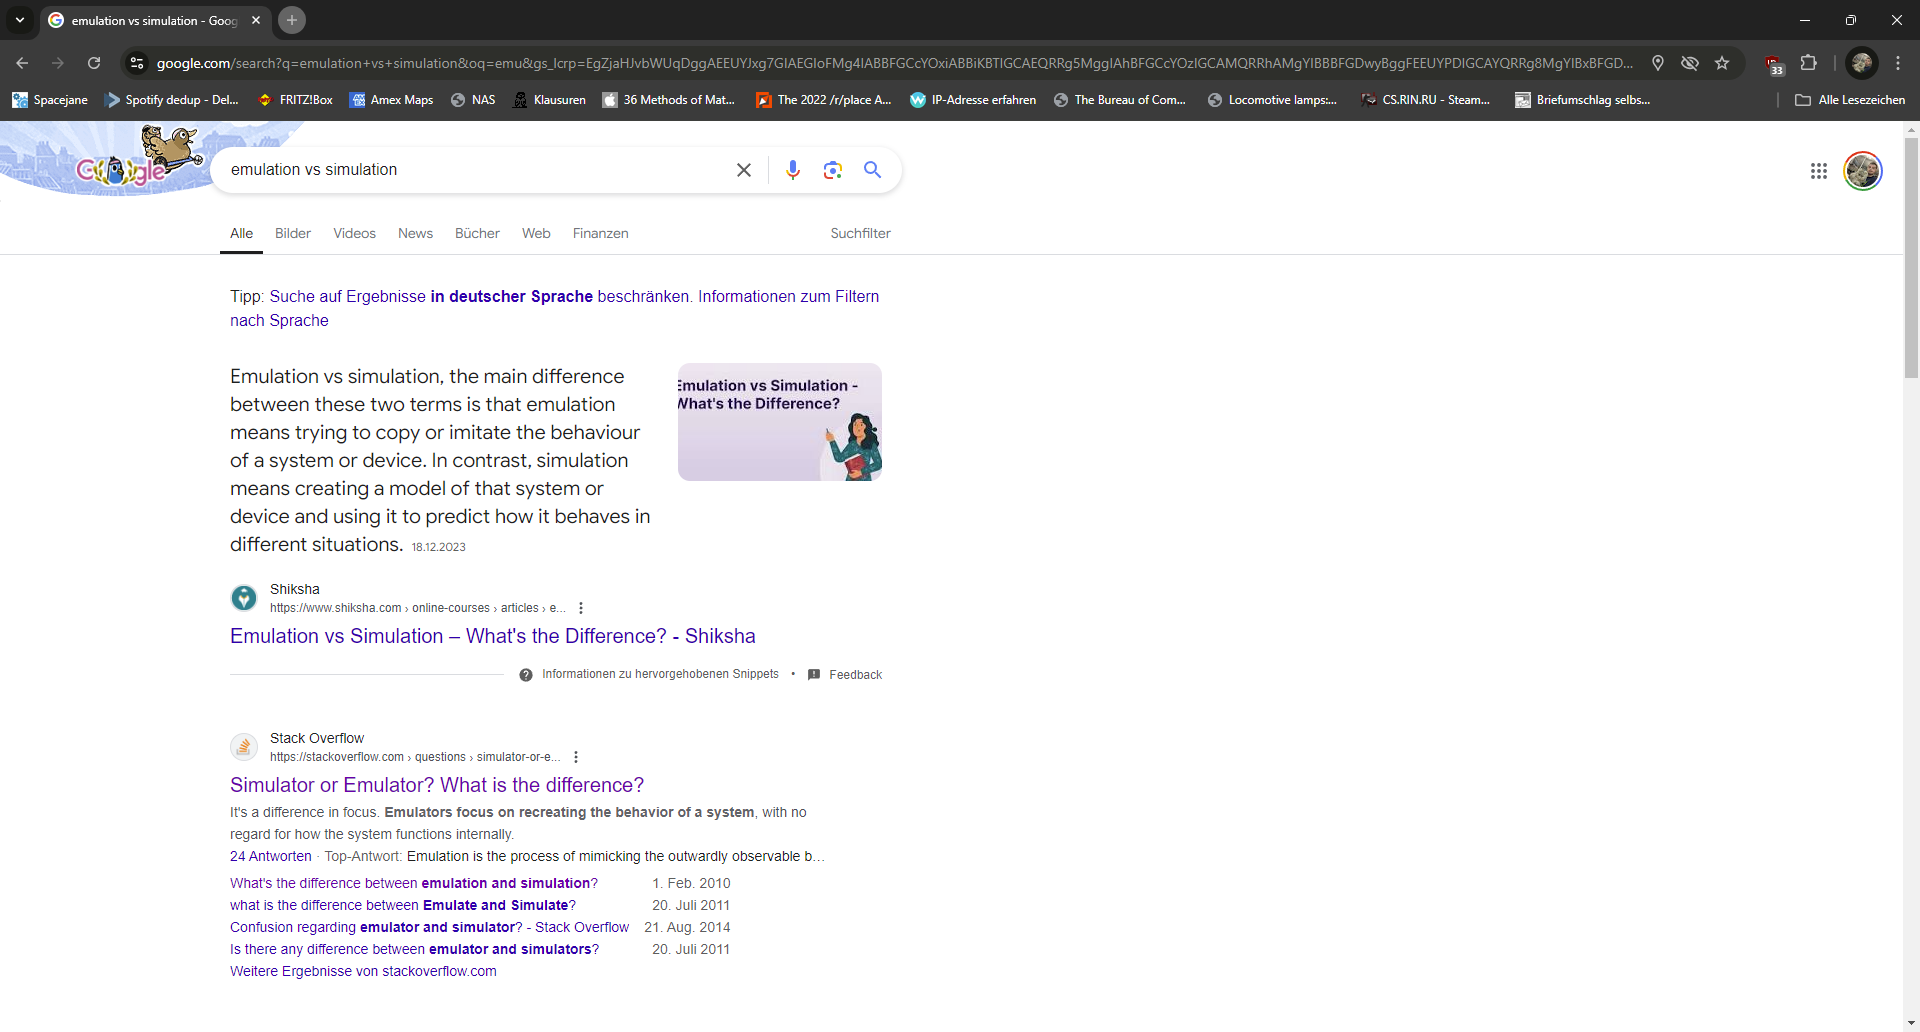
\includegraphics[width=\textwidth]{images/StackOverflow}
  \caption{The results when searching the difference between Simulation and Emulation.}
  \label{fig:Google_SO}
\end{figure}

\end{document}
